\documentclass[review]{siamart1116}

% 1. Preamble and packages
\usepackage{lipsum}
\usepackage{amsfonts}
\usepackage{graphicx}
\usepackage{epstopdf}
\usepackage{algpseudocode}
%\usepackage{algorithmic}
%\usepackage{algorithm}

\ifpdf%
  \DeclareGraphicsExtensions{.eps,.pdf,.png,.jpg}
\else
  \DeclareGraphicsExtensions{.eps}
\fi
\usepackage{amsopn}
\DeclareMathOperator{\diag}{diag}
\usepackage{booktabs}

% 2. Paper title
\newcommand{\TheTitle}{%
  Example Title
}

% 2.5. Short title for running heads (if needed)
\newcommand{\TheShortTitle}{%
  \TheTitle
}

% 3. Student Name
\newcommand{\TheName}{%
  Elena Agostini
}

% 4. Student Address
\newcommand{\TheAddress}{%
  University of Rome "La Sapienza",
  (\email{agostini@di.uniroma1.it}, \tt{http://www.uniroma1.it/}).
}

% 5. Acknowledge funding or other resources
\newcommand{\TheFunding}{%
  Project in collaboration with the CUDA team at NVIDIA\@.
}

% 6. Collaborators, such as advisor or research collaborators
\newcommand{\TheCollaborators}{%
D. Rossetti Collaborator NVIDIA,
N. Sakharnykh Collaborator NVIDIA,
M. Bernaschi PhD Supervisor
}

% ---------------------------------------------
% ---------------------------------------------
\author{\TheName\thanks{\TheAddress}}
\title{{\TheTitle}\thanks{\TheFunding}}
\headers{\TheShortTitle}{\TheName}
\ifpdf%
\hypersetup{%
  pdftitle={\TheTitle},
  pdfauthor={\TheName}
}
\fi

\begin{document}

\maketitle

\begin{center}
In collaboration with:
  {\TheCollaborators}
\end{center}
\vspace{1cm}
% ---------------------------------------------
% ---------------------------------------------

\begin{abstract}
HPGMG is a benchmark for HPC geometric multi-grid methods.
%
A multi-grid solver works on a grid having a fixed total size but
different resolutions during the execution so that the amount of computation and
communication varies significantly within the same application.
%
NVIDIA developed a CUDA version of HPGMG-FV (Finite Volume) where,
according to a threshold, finer (higher) levels are computed on the GPU
whereas coarser (lower) levels on the CPU: that hybrid scheme exploits
at their best the strengths of both platforms.
%
During the HPGMG-FV execution, there are three main communication
phases: boundaries exchange (among a variable number of cluster nodes),
interpolation (lower to higher level) and restriction (higher to lower
level). By default communications use the Message Passing Interface (MPI).

GPUDirect Async is a new technology introduced by NVIDIA in CUDA 8.0
to support mutual direct control between the GPU and the interconnect device, a
Mellanox Infiniband HCA in our case.

In this paper, we propose two optimized communication schemes involving the
GPUDirect Async technology, where the burden of the communication is
off-loaded onto the GPU itself.
%
When running a properly modified version of HPGMG-FV, where Async
technology is used for only those aforementioned communication phases,
the communication overhead reduces up to 26\% .

\end{abstract}

\begin{keywords}
  HPGMG-FV, Multi-Grid, GPU, Asynchronous Communication, GPUDirect Async
\end{keywords}

\section{Introduction}\label{sec:introduction}
%Linear solvers are probably the most common tool in scientific computing applications and can be divided in two basic classes: \emph{direct} and \emph{iterative}.
% Direct methods are usually robust, but have additional computational complexity and memory capacity requirements, while iterative solvers require minimal memory overhead and feature better computational complexity.
\emph{Multi-grid} methods are iterative methods that can deliver
linear complexity by solving elliptic PDEs %$Ax=b$
using a hierarchical approach, i.e. the solution to a hard problem (finer grid of elements) is expressed as solution to an easier problem (coarser grid of element).
There are two different types of \emph{Multi-grid} methods: algebric multi-grid (\emph{AMG}), where operator A is a sparse matrix, and geometric multi-grid (\emph{GMG}), where operator A is a stencil\footnote{Stencil codes are a class of iterative kernels which update array (generally a 2- or 3-dimensional regular grid) elements (cells) according to some fixed pattern, called stencil. The state of a cell in the next time step can be deduced from its own previous state and the states of the cells in its neighborhood.
}. While AMG method is a more general approach using an arbitrary graph, GMG method is more efficient on structured problems, since it can take advantage of the additional information from the geometric representation of the problem.

HPGMG is an example of GMG developed by Lawrence Berkeley National
Laboratory \cite{HPGMG} that is often employed also as a HPC benchmark. In particular, HPGMG-FV solves variable-coefficient elliptic problems on isotropic Cartesian grids using the finite volume method (FV) \cite{finitevolume}.
It supports high-order discretizations, and it is extremely fast and accurate; in case of multi-process execution, the workload is fairly distributed among processes: in order to improve the parallelization, each problem level is divided into several same-size boxes.

%The solution to a hard problem (a continuous problem expressed by a finer grid of elements by means of discretization) is expressed as a solution to an easier problem (coarser grid of element).

HPGMG-FV takes as input the number and the $\log_2 (size)$ of the finest level boxes, calculating the level
total size; then it obtains the size of all the other (coarse grain) levels. Every distributed level is computed with smoothing and residual operations; in particular the smoother is a stencil code and the tasks of each process are:

\begin{itemize}
\item Pack: compute the boundaries of the box and copy them inside send buffers;
\item Send: distribute the boundaries to the other processes (\emph{intra-level} communication);
\item Interior Compute: apply the stencil operator to the inner elements of the box;
\item Receive: receive boundaries from the other processes (\emph{intra-level} communication)
\item Unpack: copy (and compute) received data along box boundaries
\end{itemize}

HPGMG-FV implements an F-cycle (Figure \ref{fig:hpgmg_fcycle}) which starts at the bottom of the multi-grid hierarchy and performs multiple V-cycles (Figure \ref{fig:hpgmg_vcycle}), gradually adding finer levels. %Every V-cycle is mainly dominated by the smoothing a stencil code in HPGMG-FV case), and residual operations at the top (finer) levels.
During a V-cycle, the grid is smoothed and a residual is computed and propagated to the coarser grid. At the coarsest level, a direct solver is applied, and the solution is then iteratively interpolated to finer grids.

\begin{figure}[h]
\centering
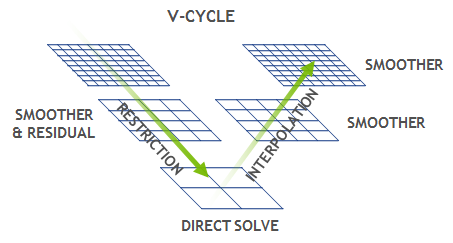
\includegraphics[scale=0.7]{hpgmg_v_cycle.png}
\caption{V-Cycle}
\label{fig:hpgmg_vcycle}
\end{figure}

The F-cycle is considered state-of-the-art in multi-grid methods and converges much faster than a conventional V-cycle.

\section{HPGMG-FV and GPUs}\label{sec:hpgmg_cuda}

NVIDIA improved the HPGMG-FV implementation \cite{HPGMG_NVIDIA} using
a hybrid solution that guarantees that each level in the F-Cycle is
executed on the most suitable architecture: if the size of a level is over a certain threshold (empirically set to 10000 elements), it is processed by the GPU, otherwise by the CPU (Figure \ref{fig:hpgmg_fcycle}).

\begin{figure}[h]
\centering
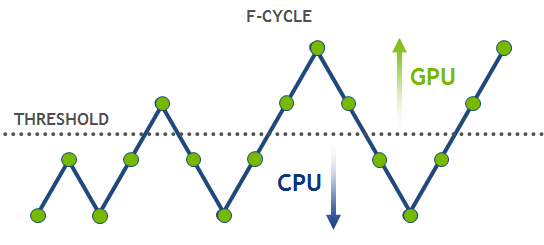
\includegraphics[scale=0.6]{hpgmg_f_cycle.png}
\caption{F-Cycle with CPU-GPU threshold}
\label{fig:hpgmg_fcycle}
\end{figure}

To leverage GPU acceleration for higher levels, the simplest way was to use device memory for compute-only buffers and host pinned memory for communication buffers.

Considering a distributed HPGMG-FV execution, we can distinguish between two different communication phases (referring to Figure \ref{fig:hpgmg_vcycle}):
\begin{enumerate}
\item \textbf{Intra-level communication}: exchange boundaries (boundary region exchange of the same level between proccesses )
\item \textbf{Inter-level communication}: restriction (moving from a finer level to a coarser level) and interpolation (moving from a coarser level to a finer level)
\end{enumerate}

The most frequent communication is the \emph{exchangeBoundaries()} executed by the smoother's
stencil code on a distributed level, that works according to Algorithm
\ref{algo:exchange_boundaries}.

\begin{algorithm}
\small
\caption{Exchange Boundaries function}
\label{algo:exchange_boundaries}
\begin{algorithmic}[1]
\For{$i$ = 1 to PROCESSES }
\State cudaMallocHost(sendBuffers$[i]$)
\State cudaMallocHost(receiveBuffers$[i]$)
\EndFor
\State ...
\Function{exchangeBoundaries}{ } \label{alg:b}
        \For{$i$ = 1 to PROCESSES }
                \State MPI\_Irecv(receiveBuffers$[i]$, \&reqs\_recv$[i]$)
        \EndFor
        \State cuda\_pack(sendBuffers)
        \State cudaDeviceSynchronize()
        \For{$i$ = 1 to PROCESSES }
                \State MPI\_Isend(sendBuffers$[i]$)
        \EndFor
        \State cuda\_interior\_compute(localBuffers)
        \State MPI\_Waitall(reqs\_recv)
        \State cuda\_unpack(receiveBuffers)
\EndFunction
\end{algorithmic}
\end{algorithm} \textit{cudaDeviceSynchronize()} is required between the CUDA kernel
pack operation and the \textit{MPI\_Isend()} to guarantee the correctness
of updated \textit{sendBuffers} (Figure \ref{fig:timeline_mpi}).
The \textit{exchangeBoundaries()} is the most used communication function during a HPGMG-FV execution.

\begin{figure}[h]
\centering
\includegraphics[scale=0.3]{timeline_mpi.png}
\caption{Synchronous \textit{exchangeBoundaries()} timeline}
\label{fig:timeline_mpi}
\end{figure}

Similarly, the other two \emph{inter-level} communication functions, i.e. restriction and interpolation, require a \textit{cudaDeviceSynchronize()} before the \textit{MPI\_Isend()}. Restriction needs an additional \textit{cudaDeviceSynchronize()} when moving from a GPU level to a CPU level.

Figure \ref{fig:hpgmg_levels} shows a simplified operations timeline
in case of a hybrid solution when moving from a coarse level (CPU) to
a fine level (GPU) and coming back to the coarse level (CPU).

\begin{figure}[h]
\centering
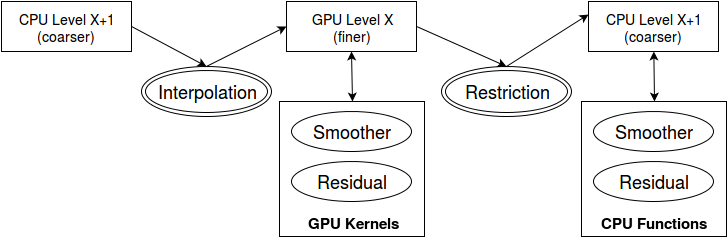
\includegraphics[scale=0.4]{hpgmg_levels.png}
\caption{F-Cycle: moving from a coarse level to a finer level and then going back to the coarse level. Restriction and interpolation play a role in case of moving from a level to another (\emph{inter-level} communication)}
\label{fig:hpgmg_levels}
\end{figure}

\iffalse
In Figure \ref{fig:hpgmg_ornl_bench} we report the enhancement obtained by the hybrid solution in a benchmark on the ORNL Titan supercomputer \cite{ornl}. For further details, please refer to \cite{HPGMG_NVIDIA}

\begin{figure}[h]
\centering
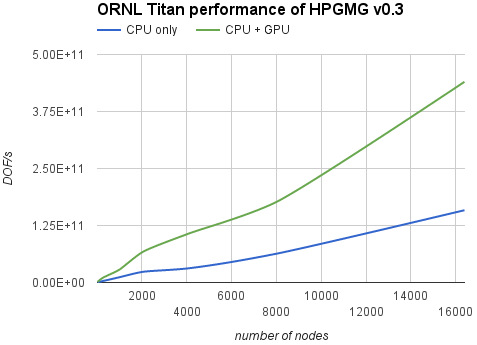
\includegraphics[scale=0.7]{hpgmg_ornl_titan_perf_cuda.png}
\caption{Performance of GPU-accelerated HPGMG on the ORNL Titan supercomputer. Results obtained by Sam Williams from Lawrence Berkeley National Lab.}
\label{fig:hpgmg_ornl_bench}
\end{figure}

\fi
Starting from that NVIDIA hybrid implementation, we have enhanced the
performance of the communication phases, which play an important role during distributed executions, using a new feature named GPUDirect Async, introduced by NVIDIA along with CUDA 8.0.
The aim of the experiment is to demonstrate how this new technology
can reduce the communication overhead in real-world distributed applications having high complexity like HPGMG-FV.


\section{GPUDirect Async}\label{sec:gpudirect_async}

GPUDirect \cite{GPUDirect} is a family of technologies aimed at
optimizing data movement respectively among GPUs (P2P) and with
third-party devices (RDMA). GPUDirect Async is a new GPUDirect
technology introduced by NVIDIA in CUDA 8.0; it allows mutual direct
control between the GPU and third party devices like Infiniband in
case of communications. The CPU can enqueue on a CUDA stream both
computation (i.e. {\em classic} CUDA kernels) and communication tasks
and go back to do useful work waiting for GPU tasks completion only
when needed. Although an in-depth explaination of the GPUDirect Async
implementation is beyond the scope of the present work, in the following we will briefly describe how it works and how it can be useful to improve HPGMG-FV performance.\\

Considering a typical multi-GPU application in case of distributed execution, a common pattern is:
\begin{itemize}
\item Work on some data using one or more CUDA kernels
\item Store data results in one or more send buffers
\item Send data
\item Wait for data from the other processes
\item Launch one or more CUDA kernels to work on received data
\end{itemize}
In Figure \ref{fig:commonmultigpu} there is a timeline of this sequence in case of Infiniband as communication technology. By leveraging GPUDirect Async, a
whole parallel computation phase can be offloaded onto a
CUDA stream, removing the CPU from the critical path, as described
in Figure \ref{fig:asyncmultigpu}.\\

\begin{figure}[h]
\centering
\includegraphics[scale=0.35]{common_multigpu.png}
\caption{Common communication pattern in Multi-GPU application timeline}
\label{fig:commonmultigpu}
\end{figure}


\begin{figure}[h]
\centering
\includegraphics[scale=0.35]{async_multigpu.png}
\caption{Communication pattern in Multi-GPU application timeline leveraged with GPUDirect Async}
\label{fig:asyncmultigpu}
\end{figure}

GPUDirect Async has two different execution models:

\begin{itemize}
\item \textbf{Stream Async model (SA)}: The one described in this Section, in which communications are enqueued into a CUDA stream;
\item \textbf{Kernel-Initiated model (KI)}: The Streaming Multiprocessors (SMs), which are in charge of executing the CUDA kernels, can directly issue communication primitives to send messages or wait for completion. %Having doorbell registers and CQs mapped as device memory addresses, a CUDA kernel thread can use simple value assignments and comparisons inside the code to ring the doorbell or poll the CQs.\\
\end{itemize}

On the top of the GPUDirect Async stack software there is LibMP, an NVIDIA open-source messaging library (similar to MPI) developed as a technology demostrator to easily deploy the GPUDirect Async technology on MPI applications. LibMP API enables the use of asynchronous communication in both SA and KI models and presents also a third model that is totally synchronous for performance comparison purposes.
HPGMG-FV communication pattern is quite similar to the one in Figure
\ref{fig:commonmultigpu}, therefore we modified the communication part
to leverage GPUDirect Async.\\

For the following benchmarks, we used two different environments.
The first one (E1) is composed by two standard 2U Xeon based
servers, each one with a Mellanox dual-port FDR Connect-Infiniband HCA and a single
Tesla K40m (boost clocks set to 875 MHz), running RHEL 6.6 and a
pre-release version of the GPU display driver with CUDA 8.0 RC and OpenMPI version 1.10.3.

The second one (E2) is the Wilkes HPC cluster at the Cambridge
University, UK \cite{wilkes}. The system consists of 128 Dell T620 servers, 256 NVIDIA Tesla K20c GPUs interconnected by 256 Mellanox Connect Infiniband cards, having the CUDA 8.0 Toolkit, display driver 367.44 and OpenMPI version 1.10.3. We had a reservation of 16 nodes to benchmark our HPGMG-FV Async solution.

\section{HPGMG-FV Async}\label{sec:hpgmg_async}

We used both SA and KI models trying to reduce, during communications, the number of
\textit{cudaDeviceSynchronize()}, which slow down performance, and to
hide kernel launches latency. We implemented also a synchronous
version with the LibMP functions to make a comparison with the similar synchronous MPI functions.
For our benchmarks we considered the GSRB smoother usign a fixed number of 8 boxes for each process, varying the $\log_2 (size)$ parameter between 4 and 7.

In Figure \ref{fig:hpgmg_gai_ivy} there is
a first benchmark with 2 processes on the E1 environment, considering
the times of GPU levels only. Both LibMP synchronous and asynchronous
models are faster than the original MPI implementation and, in particular,
Kernel-Initiated model offers a time gain up to 13\% .

\begin{figure}[h]
\centering
\includegraphics[scale=0.35]{hpgmg_gain_ivy.png}
\caption{HPGMG-FV time gain LibMP models on MPI, GPU levels only, E1 environment, 2 processes}
\label{fig:hpgmg_gai_ivy}
\end{figure}

\subsection{Stream Asynchronous model implementation}\label{sec:sahpgmg}

Algorithm \ref{algo:exchange_boundaries_async} shows the pseudo-code
of the \textit{exchangeBoundariesAsync()}.

\begin{algorithm}
\small
\caption{Exchange Boundaries Stream Async function}
\label{algo:exchange_boundaries_async}
\begin{algorithmic}[1]
\For{$i$ = 1 to PROCESSES }
\State cudaMallocHost(sendBuffers$[i]$)
\State cudaMallocHost(receiveBuffers$[i]$)
\EndFor
\State ...
\Function{exchangeBoundariesStreamAsync}{stream} \label{alg:a}
        \For{$i$ = 1 to PROCESSES }
                \State mp\_irecv(receiveBuffers$[i]$, \&receiveDescriptors$[i]$)
        \EndFor
        \State cuda\_pack(sendBuffers, stream)
        \For{$i$ = 1 to PROCESSES }
                \State mp\_isend\_on\_stream(sendBuffers$[i]$, \&sendDescriptors$[i]$, stream)
        \EndFor
        \State cuda\_interior\_compute(localBuffers, stream)
        \State mp\_wait\_all\_on\_stream(receiveDescriptors, stream)
        \State cuda\_unpack(receiveBuffers, stream)
        \State mp\_wait\_all\_on\_stream(sendDescriptors, stream)
\EndFunction
\end{algorithmic}
\end{algorithm}

The \textit{cudaDeviceSynchronize()} between the pack and the send operations is no more required. The CUDA stream is responsible for:

\begin{enumerate}
\item Packing data in the \textit{sendBuffers} by means of the \textit{cuda\_pack()} kernel
\item Triggering the send operations (send WQEs have been previously posted in the QP by the CPU)
\item Executing the \textit{cuda\_interior\_compute()} kernel
\item Waiting for the receive completion
\item Reading the received data (\textit{receiveBuffers}) with the \textit{cuda\_unpack()} kernel
\end{enumerate}

%Similar considerations can be done for \textit{restriction()} and \textit{interpolation()} functions.
Considering a similar implementation for restriction and interpolation, since the asynchronous communications are used only in case of GPU levels, a single \textit{cudaDeviceSynchronize()} is required during restriction when moving from a GPU level to a CPU level. During GPU levels, the CPU can launch all the CUDA kernels without waiting, hiding the kernel launch times (timeline in Figure \ref{fig:timeline_async}).

\begin{figure}[h]
\centering
\includegraphics[scale=0.4]{timeline_async.png}
\caption{\textit{exchangeBoundariesStreamAsync()} timeline}
\label{fig:timeline_async}
\end{figure}

%
In Figure \ref{fig:hpgmg_gain_sa_wilkes} the $y$ axis shows the
performance improvement of the GPU levels using the Stream Async
implementation  with respect to the standard MPI mode in the E2 environment (Wilkes HPC) using up to 16 processes.
%
The maximum gain (about 24\%) is reached in case of $\log_2(size)=4$
with 2 processes. The bigger is the box size, the more the performance
gain decreases, because the message size grows with the box size,
therefore comunication overhead becomes less important.

\begin{figure}[htb]
\centering
\includegraphics[scale=0.5]{hpgmg_gain_sa_wilkes.png}
\caption{HPGMG-FV time gain Stream Async on MPI, GPU levels only, E2 environment, up to 16 processes}
\label{fig:hpgmg_gain_sa_wilkes}
\end{figure}

\subsection{Kernel-Initiated model implementation}\label{sec:kihpgmg}

The algorithm from the CPU point of view is extremely simple (Algorithm \ref{algo:exchange_boundaries_gpu} and timeline in Figure \ref{fig:gpu_initiated_timeline}): it must prepare send/receive descriptors and launch a single CUDA kernel in which GPU will overlap, as much as possible, all the \textit{exchangeBoundaries()} operations.

\begin{algorithm}
\small
\caption{Exchange Boundaries kernel-initiated function}
\label{algo:exchange_boundaries_gpu}
\begin{algorithmic}[1]
\For{$i$ = 1 to PROCESSES }
\State cudaMallocHost(sendBuffers$[i]$)
\State cudaMallocHost(receiveBuffers$[i]$)
\EndFor
\State ...
\Function{exchangeBoundariesKernelInitiated}{stream}
        \For{$i$ = 1 to PROCESSES }
                \State mp\_irecv(receiveBuffers$[i]$, \&receiveDescriptors$[i]$)
        \EndFor
        \For{$i$ = 1 to PROCESSES }
                \State mp\_send\_prepare(\&sendDescriptors$[i]$)
        \EndFor
        \State cuda\_compute\_exchange\_kernel(receiveDescriptors, sendDescriptors, stream)
        \State mp\_wait\_all\_on\_stream(sendDescriptors, stream)
\EndFunction
\end{algorithmic}
\end{algorithm}

\begin{figure}[h]
\centering
\includegraphics[scale=0.35]{timeline_gpu.png}
\caption{\textit{exchangeBoundariesKernelInitiated()} timeline}
\label{fig:gpu_initiated_timeline}
\end{figure}


The complexity is moved to \textit{cuda\_compute\_exchange\_kernel()} which
in a sense employs both tasks (different blocks deal with different tasks)
and data (threads in the same block cooperatively work on the same task)
parallelism in the same kernel.

According to previous observations about the HPGMG-FV smoother, we can
distringuish three different groups of independent operations:
%\begin{itemize}
\lbrack pack, send\rbrack,
\lbrack interior compute\rbrack,
\lbrack receive, unpack\rbrack.
%\end{itemize}
%
The idea is to assign these tasks to the different blocks of a single CUDA
kernel.
%
Basically, the \textit{cuda\_compute\_exchange\_kernel()} needs $N+M+1$
blocks in a mono-dimensional grid, where N is the number of blocks required
by the \textit{cuda\_pack()} and \textit{cuda\_interior\_compute()} and M
is the number of blocks required by \textit{cuda\_unpack()} plus 1 block,
used to receive data as shown in Figure \ref{fig:gpu_initited}.
%

\begin{figure}[h]
\centering
\includegraphics[scale=0.4]{hpgmg_gpu.png}
\caption{cuda\_compute\_exchange\_kernel()}
\label{fig:gpu_initited}
\end{figure}


We use atomic memory operations to pick each thread block
\footnote{There is no guarantee about the order blocks are scheduled by the
  GPU HW.} and to assign it to the right task preventing
dead-locks.

Receiving is a time critical task, so the first \textit{receiver} thread
block is used to wait for incoming messages. In particular each thread
\textit{polls} on the receive completion queue associated to each remote
node.
%
All the \textit{sender} blocks from the second to the $N+1$-th are assigned
to the \lbrack pack, send\rbrack~group of operations plus the \lbrack
interior compute\rbrack.
%
Finally, the remaining M \textit{unpacker} blocks wait for the
\textit{receiver} block to signal that all incoming data have been received,
before unpacking them.


\begin{figure}[h]
\centering
\includegraphics[scale=0.4]{global_lock.png}
\caption{inter-block barrier}
\label{fig:global_lock}
\end{figure}

An inter-block barrier scheme is used to synchronize the \textit{receiver}
and the \textit{unpacker} blocks, as explained in Figure
\ref{fig:global_lock}. Thread 0 of each \textit{unpacker}
block waits for thread 0 of the
\textit{receiver} block to set a global memory variable equal to 1, whereas the
remaining threads move to the \textit{\_\_syncthreads()} barrier.
%
When that happens (after the receive completion), all threads 0 in the
\textit{unpacker} blocks will reach the matching \textit{\_\_syncthreads()}
barrier and then start to unpack the received data.




%\begin{figure*}
%\includegraphics[width=\textwidth]{hpgmg_gpu.png}
%\subfloat[\textit{exchangeBoundariesKernelInitiated()} timeline]{\includegraphics[width=2.8in]{timeline_gpu.png}}
%\hfil
%\subfloat[cuda\_compute\_exchange\_kernel()]{\includegraphics[width=4.1in]{hpgmg_gpu.png}}
%\caption{kernel-initiated mode}
%\label{fig:gpu_initited}
%\end{figure*}



When using Kernel-Initiated model, to avoid dead-locks the \textit{receiver}
task must not prevent the \textit{sender} task from starting or
progressing: there must be always at least one block waiting for receiving and an other block executing the send.

\begin{figure}[h]
\centering
\includegraphics[scale=0.5]{hpgmg_gain_ki_wilkes.png}
\caption{HPGMG-FV time gain Kernel-Initiated on MPI, GPU levels only, E2 environment, up to 16 processes}
\label{fig:hpgmg_gain_ki_wilkes}
\end{figure}

We performed the same tests as in the previous Section (on the E2 environment using up to 16 processes, Figure \ref{fig:hpgmg_gain_ki_wilkes}) to evaluate Kernel-Initiated implementation performance. The maximum gain is 26\% in case of 2 processes with $\log_2(size)=4$ box size and, generally speaking, the performance with Kernel-Initiated model is always better than Stream Async model performance.

%When using kernel-initiated mode, it is very important that the receive (or wait for receive) operation is not preventing the send, otherwise you will have a deadlock: you must always have at least a block waiting for receive and an other block executing the send.
%For example, having a GPU with 15 SM, if the first one is waiting on the receive and the others 14 are waiting on the global lock for the receive completion, the \lbrack pack, send\rbrack \ operations will never occur.

\subsection{Communication-only improvement}\label{sec:comm_only}

To better evaluate the GPUDirect Async benefits, in Figure \ref{}
there is the gain in both SA and KI models considering communication times only.\\

----- FIGURA -----\\

\subsection{Jacobi smoother}\label{sec:jacobi}

We benchmarked all the solution discussed using a different smoother, i.e. the Jacobi smoother, reporting in Figure \ref{} the gain of SA and KI model on MPI in the E2 environment.



% An example of a floating figure using the graphicx package.
% Note that \label must occur AFTER (or within) \caption.
% For figures, \caption should occur after the \includegraphics.
% Note that IEEEtran v1.7 and later has special internal code that
% is designed to preserve the operation of \label within \caption
% even when the captionsoff option is in effect. However, because
% of issues like this, it may be the safest practice to put all your
% \label just after \caption rather than within \caption{}.
%
% Reminder: the "draftcls" or "draftclsnofoot", not "draft", class
% option should be used if it is desired that the figures are to be
% displayed while in draft mode.
%
%\begin{figure}[!t]
%\centering
%\includegraphics[width=2.5in]{myfigure}
% where an .eps filename suffix will be assumed under latex,
% and a .pdf suffix will be assumed for pdflatex; or what has been declared
% via \DeclareGraphicsExtensions.
%\caption{Simulation results for the network.}
%\label{fig_sim}
%\end{figure}

% Note that the IEEE typically puts floats only at the top, even when this
% results in a large percentage of a column being occupied by floats.


% An example of a double column floating figure using two subfigures.
% (The subfig.sty package must be loaded for this to work.)
% The subfigure \label commands are set within each subfloat command,
% and the \label for the overall figure must come after \caption.
% \hfil is used as a separator to get equal spacing.
% Watch out that the combined width of all the subfigures on a
% line do not exceed the text width or a line break will occur.
%
%\begin{figure*}[!t]
%\centering
%\subfloat[Case I]{\includegraphics[width=2.5in]{box}%
%\label{fig_first_case}}
%\hfil
%\subfloat[Case II]{\includegraphics[width=2.5in]{box}%
%\label{fig_second_case}}
%\caption{Simulation results for the network.}
%\label{fig_sim}
%\end{figure*}
%
% Note that often IEEE papers with subfigures do not employ subfigure
% captions (using the optional argument to \subfloat[]), but instead will
% reference/describe all of them (a), (b), etc., within the main caption.
% Be aware that for subfig.sty to generate the (a), (b), etc., subfigure
% labels, the optional argument to \subfloat must be present. If a
% subcaption is not desired, just leave its contents blank,
% e.g., \subfloat[].


% An example of a floating table. Note that, for IEEE style tables, the
% \caption command should come BEFORE the table and, given that table
% captions serve much like titles, are usually capitalized except for words
% such as a, an, and, as, at, but, by, for, in, nor, of, on, or, the, to
% and up, which are usually not capitalized unless they are the first or
% last word of the caption. Table text will default to \footnotesize as
% the IEEE normally uses this smaller font for tables.
% The \label must come after \caption as always.
%
%\begin{table}[!t]
%% increase table row spacing, adjust to taste
%\renewcommand{\arraystretch}{1.3}
% if using array.sty, it might be a good idea to tweak the value of
% \extrarowheight as needed to properly center the text within the cells
%\caption{An Example of a Table}
%\label{table_example}
%\centering
%% Some packages, such as MDW tools, offer better commands for making tables
%% than the plain LaTeX2e tabular which is used here.
%\begin{tabular}{|c||c|}
%\hline
%One & Two\\
%\hline
%Three & Four\\
%\hline
%\end{tabular}
%\end{table}


% Note that the IEEE does not put floats in the very first column
% - or typically anywhere on the first page for that matter. Also,
% in-text middle ("here") positioning is typically not used, but it
% is allowed and encouraged for Computer Society conferences (but
% not Computer Society journals). Most IEEE journals/conferences use
% top floats exclusively.
% Note that, LaTeX2e, unlike IEEE journals/conferences, places
% footnotes above bottom floats. This can be corrected via the
% \fnbelowfloat command of the stfloats package.


\section{Conclusions}

We presented the performance of a GPU accelerated multi-node
implementation of the HPGMG-FV benchmark using the recently introduced
NVIDIA GPUDirect Async technology, demonstrating how the use of asynchronous communications,
according to different execution models, can be useful for this particular class of applications.
%
GPUDirect Async has been
released with CUDA 8.0 whereas Infiniband network support for
Async comes in the form of a new set of experimental
OFED verbs (Mellanox OFED 3.4 plus updates in \cite{libmlx5_async})
and a mid layer abstraction library \cite{libgdsync} as BSD.
%
In the near future,  we are going to test
asychronous HPGMG-FV, and other similar proxy applications, using a higher number of nodes to
better evaluate the scalability of the GPUDirect technology..

\bibliographystyle{siamplain}
\begin{thebibliography}{1}

%\bibitem{IEEEhowto:kopka}
%H.~Kopka and P.~W. Daly, \emph{A Guide to \LaTeX}, 3rd~ed.\hskip 1em plus
%  0.5em minus 0.4em\relax Harlow, England: Addison-Wesley, 1999.

\bibitem{GPUDirect} \emph{GPUDirect family} \relax  https://developer.nvidia.com/gpudirect

\bibitem{mellanoxgdr} \emph{Mellanox GDR}  \relax http://www.mellanox.com/page/products\_dyn?product\_family=116

\bibitem{rdmamellnox} \emph{IB Verbs RDMA programming guide}. \relax http://www.mellanox.com/related-docs/prod\_software/RDMA\_Aware\_Programming\_user\_manual.pdf

\bibitem{HPGMG} HPGMG https://hpgmg.org

\bibitem{HPGMG_NVIDIA} N. ~Sakharnykh \emph{High-Performance Geometric Multi-Grid with GPU Acceleration}. \relax https://devblogs.nvidia.com/parallelforall/high-performance-geometric-multi-grid-gpu-acceleration

\bibitem{finitevolume} \emph{Finite Volume method}. \relax https://en.wikipedia.org/wiki/Finite\_volume\_method

\bibitem{fullmultigrid} \emph{Full MultiGrid method}. \relax https://en.wikipedia.org/wiki/Multigrid\_method

\bibitem{ornl} \emph{ORNL Titan supercomputer}. \relax https://www.olcf.ornl.gov/titan

\bibitem{wilkes} \emph{Wilkes HPC Cambridge, UK}. \relax www.hpc.cam.ac.uk

\bibitem{exmatex} \emph{ExMaTex}. \relax http://www.exmatex.org/comd.html

\bibitem{libmlx5_async} \emph{GPUDirect libmlx5}. \relax https://github.com/gpudirect/libmlx5

\bibitem{libgdsync} \emph{GPUDirect libgdsync}. \relax https://github.com/gpudirect/libgdsync

\end{thebibliography}

%\bibliography{references}

\end{document}
